\documentclass[15pt,a5paper,reqno]{article}
\usepackage{hyperref}
\usepackage[warn]{mathtext}
\usepackage[utf8]{inputenc}
\usepackage[T2A]{fontenc}
\usepackage[russian]{babel}
\usepackage{amssymb, amsmath, multicol}
\usepackage{graphicx}
\usepackage[shortcuts,cyremdash]{extdash}
\usepackage{wrapfig}
\usepackage{gensymb}
\usepackage{floatflt}
\usepackage{lipsum}
\usepackage{verbatim}
\usepackage{concmath}
\usepackage{euler}
\usepackage{xcolor}
\usepackage{etoolbox}
\usepackage{fancyhdr}
\usepackage{subfiles}
\usepackage{enumitem}
\usepackage{amsthm}
\usepackage{indentfirst}
\usepackage{import}
\usepackage{multirow}
\usepackage{hhline}

\DeclareMathOperator{\sign}{sign}

\RequirePackage[ left     = 1cm,
                 right    = 1cm,
                 top      = 2.0cm,
                 bottom   = 1.25cm,
                 includefoot,
                 footskip = 1.25cm ]{geometry}
                 
\setlength{\parskip}{ .5em plus .15em minus .08em }
\renewcommand {\baselinestretch}{ 1.07 }

\fancyhf{} % clear existing header/footer entries

\renewcommand{\footrulewidth}{ .0em }
\fancyfoot[C]{\texttt{\textemdash~\thepage~\textemdash}}

\makeatletter
\patchcmd\l@section{%
  \nobreak\hfil\nobreak
}{%
  \nobreak
  \leaders\hbox{%
    $\m@th \mkern \@dotsep mu\hbox{.}\mkern \@dotsep mu$%
  }%
  \hfill
  \nobreak
}{}{\errmessage{\noexpand\l@section could not be patched}}
\makeatother
\parindent = 1cm % отступ при красной строке⏎
\pagestyle{fancy}    
\renewcommand\qedsymbol{$\blacksquare$}

\newcommand{\when}[2]{
  \left. #1 \right|_{#2} \hspace
}
\renewcommand{\kappa}{\varkappa}
\RequirePackage{caption2}
\renewcommand\captionlabeldelim{}
\newcommand*{\hm}[1]{#1\nobreak\discretionary{}

\DeclareSymbolFont{T2Aletters}{T2A}{cmr}{m}{it}
{\hbox{$\mathsurround=0pt #1$}}{}}
% Цвета для гиперссылок
\definecolor{linkcolor}{HTML}{000000} % цвет ссылок
\definecolor{urlcolor}{HTML}{799B03} % цвет гиперссылок
 
\hypersetup{pdfstartview=FitH,  linkcolor=linkcolor,urlcolor=urlcolor, colorlinks=true}


\begin{document}

% НАЧАЛО ТИТУЛЬНОГО ЛИСТА
\begin{center}
  {\small ФЕДЕРАЛЬНОЕ ГОСУДАРСТВЕННОЕ АВТОНОМНОЕ ОБРАЗОВАТЕЛЬНОЕ\\ УЧРЕЖДЕНИЕ ВЫСШЕГО ОБРАЗОВАНИЯ\\ МОСКОВСКИЙ ФИЗИКО-ТЕХНИЧЕСКИЙ ИНСТИТУТ\\ (НАЦИОНАЛЬНЫЙ ИССЛЕДОВАТЕЛЬСКИЙ УНИВЕРСИТЕТ)\\ ФИЗТЕХ-ШКОЛА РАДИОТЕХНИКИ И КОМПЬЮТЕРНЫХ ТЕХНОЛОГИЙ}\\
  \hfill \break
  \hfill \break
  \hfill \break
  \Huge{Работа 3.4.1. \\ Диа- и парамагнетики}\\
\end{center}

\hfill \break
\hfill \break
\hfill \break
\hfill \break
\hfill \break
\hfill \break
\hfill \break
\hfill \break

\begin{flushright}
  \normalsize{Работу выполнил:}\\
  \normalsize{\textbf{Долгов Александр Алексеевич, группа Б01-106}}\\
\end{flushright}

\begin{center}
  \normalsize{\textbf{Долгопрудный, 2022}}
\end{center}

\thispagestyle{empty} % выключаем отображение номера для этой страницы

% КОНЕЦ ТИТУЛЬНОГО ЛИСТА

\newpage
\thispagestyle{plain}
\tableofcontents
\thispagestyle{plain}
\newpage

\section{Аннотация}

    В данной работе измеряется магнитная восприимчивость диа- и парамагнетиков методом Гюи.
	
\section{Теоретические сведения}

    Магнитная восприимчивость тел может быть определена путём измерения сил, которые действуют на тела в магнитном поле. Существуют два классических метода таких измерений: метод Фарадея и метод Гюи. В методе Фарадея исследуемые образцы, имеющие форму маленьких шариков, помещаются в область сильно неоднородного магнитного поля и измеряется сила, действующая на образец. В методе Гюи используется тонкий и длинный стержень, один из концов которого помещают в зазор электромагнита, а другой конец -- вне зазора, где величиной магнитного поля можно пренебречь. В данной работе использовался метод Гюи.

    Найдём выражение для магнитной силы, действующей на образец, помещённый в зазор электромагнита. Пусть площадь образца равна $S$, его магнитная проницаемость -- $\mu$, а индукция поля в зазоре равна $B$.

    
    \begin{wrapfigure}{r}{0.35\textwidth}
        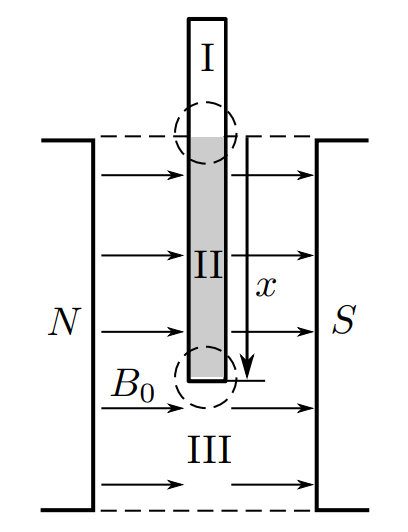
\includegraphics[width = 0.35\textwidth]{images/stick.png}
        \begin{center}
            \textbf{Рисунок 1.}
        \end{center}
    \end{wrapfigure}
    Расчёты проведём энергетическим методом. Сила, действующая на образец со стороны магнитного поля при постоянном токе в обмотке электромагнита может быть найдена по формуле:
    \begin{equation*}
        F = \left(\frac{\partial W_m}{\partial x}\right)_I,
    \end{equation*}
    где ось Ox направлена внутрь электромагнита. Магнитная энергия рассчитывается по формуле
    \begin{equation*}
    W_m=\frac{1}{2}\iiint HBd\,V = \frac{1}{2\mu_0}\iiint\frac{B^2}{\mu}d\,V,
    \end{equation*}
    где интеграл распространён на всё пространство. При смещении образца магнитная энергия меняется только в области зазора (в объёме $Sdx$), а около верхнего конца стержня остаётся неизменной, поскольку магнитного поля там практически нет. Принимая поле внутри стержня равным измеренному нами полю в зазоре $ B $, получим
    \[dW_m = dW_m^{\text{обр}} + dW_m^{зазор} = \frac{1}{2\mu_0}\frac{B_2^2}{\mu}Sdx - \frac{1}{2\mu_0}B_3^2 Sdx = \]
    \[= \frac{1}{2\mu_0}\mu B_0^2Sdx - \frac{1}{2\mu_0}B_0^2 Sdx = \frac{\mu - 1}{2\mu_0}B_0^2Sdx\]
    Следовательно, на образец действует сила (в проекции на ось Ox):
    \begin{equation}\label{force}
    \boxed{F_x = \frac{\chi}{2\mu_0}B^2S}
    \end{equation}
    Направление этой силы зависит от знака $\chi$: образцы из парамагнитных материалов $( \chi > 0)$ втягиваются в зазор электромагнита, а диамагнитные образцы $(\chi < 0)$ выталкиваются из него.
    
\section{Экспериментальная установка}

    Схема установки изображена на Рисунке 1. Магнитное поле создаётся в зазоре электромагнита, питаемого постоянным током. Это поле можно считать однородным, поскольку диаметр полюсов электромагнита значительно превосходит ширину зазора.

    \begin{center}
        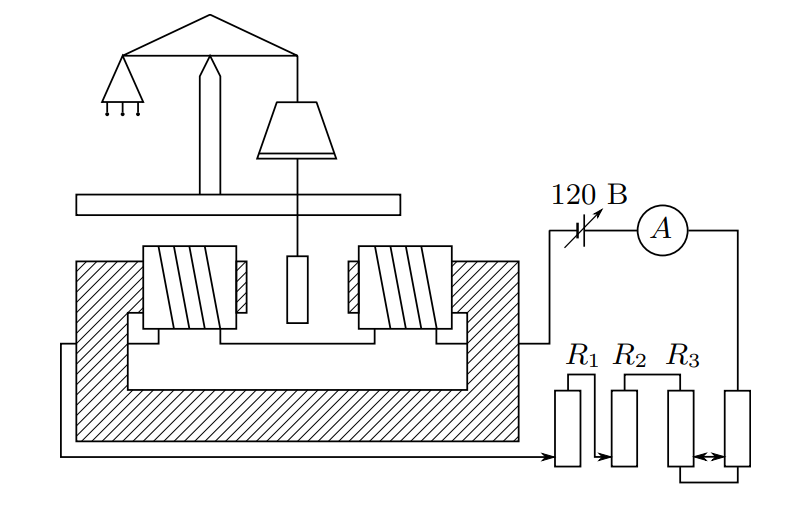
\includegraphics[width = \textwidth]{images/picture_1.png}
        \textbf{Рисунок 1. Схема экспериментальной установки}
    \end{center}

    Установка связи между индукцией магнитного поля в зазоре электромагнита и силой тока в его обмотках (градуировка электромагнита) производится при помощи милливеберметра или датчика эффекта Холла.

    При измерениях образцы поочерёдно подвешиваются к аналитическим весам так, что один конец образца оказывается в зазоре электромагнита, а другой - вне зазора. При помощи этих весов определяется сила, действующая на образец со стороны магнитного поля.
    
\section{Приборы и инструментальные погрешности}

    \noindent\textbf{Амперметр:}\\
        Абсолютная погрешность: $\sigma_I = 0.005 I + 0.02$, $[I] = \text{ А}$

    \noindent\textbf{Милливеберметр:}\\
        Абсолютная погрешность: $\sigma_{\Phi} = 0.015\Phi + 0.02$, $[\Phi] = \text{ мВб}$

    \noindent\textbf{Весы:}\\
        Абсолютная погрешность: $\sigma_{m} = 0.5\text{ мг}$

    \noindent\textbf{Штангенциркуль:}\\
        Абсолютная погрешность: $\sigma_{d} = 0.05\text{ мм}$

\section{Измерения и обработка их результатов}

    \subsection{Калибровка электромагнита}

        Для калибровки электромагнита было проведено 16 измерений потока вектора магнитной индукции через катушку и тока, протекающего по ней. Поскольку поток прямо пропорционален $B$, то была найдена зависимость $B(I)$. Результаты измерений приведены в \hyperlink{table_1}{Таблице 1}. По этим данным также построен \hyperlink{graph_1}{График 2}. Поскольку теория предсказывает, что модуль магнитной индукции $B$ прямо пропорционален току $I$, то точки на графике аппроксимировались прямой линией по методу $\chi$-квадрат.

        Пусть зависимость $B(I)$ аппроксимируется прямой $B = kI$, тогда из метода $\chi$-квадрат получаем, что:
        \begin{equation}\label{k}
            k = (305 \pm 5)\frac{\text{мТл}}{\text{А}}
        \end{equation}

    \subsection{Определение магнитной восприимчивости}

        В зазор электромагнита подвешивалось 2 образца: из алюминия и из меди. Для каждого из этих образцов измерялись сила, действующая на него, и ток, текущий через катушки электромагнита. По измеренной силе тока с помощью формулы \eqref{k} находилась величина $B^2$ Погрешность величины $B^2$ вычислялась по формуле:
        \begin{equation*}
            \sigma_{B^2} = 2B\sigma_{kI} = 2B\sqrt{\left(\frac{\sigma{k}}{k}\right)^2 + \left(\frac{\sigma{I}}{I}\right)^2}
        \end{equation*}
        Результаты измерений приведены в \hyperlink{table_2}{Таблице 2}. По этим данным также построены \hyperlink{graph_al}{График 2 (алюминий)}, \hyperlink{graph_cu}{График 3 (медь)} и \hyperlink{graph_mix}{График 4 (оба материала на одном графике)}.

        Экспериментальные зависимости были аппроксимированы прямыми по методу $\chi$-квадрат. Пусть зависимость $|\Delta P| (B^2)$ задаётся уравнением $|\Delta P| = \tilde k B^2$, тогда получаем, что:
        \begin{equation}
            \tilde k_{Al} = (550 \pm 20) \frac{\text{мкН}}{\text{Тл}^2}
        \end{equation}
        \begin{equation}
            \tilde k_{Cu} = (220 \pm 11) \frac{\text{мкН}}{\text{Тл}^2}
        \end{equation}
        Также были измерены диаметры образцов:
        \begin{equation*}
            d_{Al} = d_{Cu} = (10.00 \pm 0.05) мм
        \end{equation*}
        Из формулы \eqref{force} получаем способ вычисления магнитной восприимчивости:
        \begin{equation*}
            \chi = \frac{2\mu_0}{S}\tilde k
        \end{equation*}
        Если выразить площадь сечения образцов, через их диаметры $d$, то получим формулу, пригодную для вычислений:
        \begin{equation}\label{final}
            \boxed{\chi = \frac{8\mu_0}{\pi}\frac{\tilde k}{d^2}}
        \end{equation}
        Из формулы \eqref{final} ясно, что погрешность магнитной восприимчивости находится по формуле:
        \begin{equation*}
            \sigma_{\chi} = \chi\sqrt{\left(\frac{\sigma_{\tilde k}}{\tilde k}\right)^2 + 2\left(\frac{\sigma_d}{d}\right)^2}
        \end{equation*}
        Окончательно получаем:
        \begin{equation*}
            \chi_{Al} = (176 \pm 7)\cdot 10^{-7}
        \end{equation*}
        \begin{equation*}
            \chi_{Cu} = (70 \pm 4)\cdot 10^{-7}
        \end{equation*}
        
    
\section{Вывод}

        
    
\newpage
\section{Приложения}

    \subsection{Таблицы}

    \noindent\hypertarget{table_1}{\textbf{Таблица 1. Зависимость магнитного потока через катушку от тока в ней.}}
    \begin{center}
        \begin{tabular}{|c|c|c|c|c|c|}
        \hline
        I, А & $\sigma_I$, А & $\Phi$, мВб & $\sigma_{\Phi}$, мВб & B, мТл & $\sigma_B$, мТл  \\ \hline\hline
        0.23 & 0.02          & 0.50        & 0.01                 & 69     & 1  \\ \hline
        0.44 & 0.02          & 1.00        & 0.02                 & 139    & 2  \\ \hline
        0.57 & 0.02          & 1.20        & 0.02                 & 167    & 3  \\ \hline
        0.71 & 0.02          & 1.60        & 0.02                 & 222    & 3  \\ \hline
        0.86 & 0.02          & 1.90        & 0.03                 & 264    & 4  \\ \hline
        1.02 & 0.03          & 2.30        & 0.03                 & 319    & 5  \\ \hline
        1.23 & 0.03          & 2.75        & 0.04                 & 382    & 6  \\ \hline
        1.37 & 0.03          & 3.05        & 0.05                 & 424    & 6  \\ \hline
        1.51 & 0.03          & 3.40        & 0.05                 & 472    & 7  \\ \hline
        1.65 & 0.03          & 3.70        & 0.06                 & 514    & 8  \\ \hline
        1.84 & 0.03          & 4.05        & 0.06                 & 563    & 8  \\ \hline
        1.96 & 0.03          & 4.30        & 0.06                 & 597    & 9  \\ \hline
        2.12 & 0.03          & 4.60        & 0.07                 & 639    & 10 \\ \hline
        2.29 & 0.03          & 4.90        & 0.07                 & 681    & 10 \\ \hline
        2.38 & 0.03          & 5.10        & 0.08                 & 708    & 11 \\ \hline
        2.41 & 0.03          & 5.15        & 0.08                 & 715    & 11 \\ \hline
        \end{tabular}
    \end{center}

    \noindent\hypertarget{table_2}{\textbf{Таблица 2. Зависимость силы, действующей на образец от индукции магнитного поля.}}
    \begin{center}
        \begin{tabular}{|c|c|c|c|c|c|c|}
        \hline
        \multicolumn{2}{|c|}{$|\Delta P$|, мкН} & \multirow{2}{*}{$\sigma_{\Delta P}$, мкН} & \multirow{2}{*}{I, А} & \multirow{2}{*}{$\sigma_I$, А} & \multirow{2}{*}{$B^2$, $\text{Тл}^2$} & \multirow{2}{*}{$\sigma_{B^2}$, $\text{Тл}^2$}\\ \hhline{--~~~~~}
        Al  & Cu  &                    &       &      &      &   \\ \hline\hline

        20  & 10  & \multirow{6}{*}{5} & 0.5   & 0.02 & 0.023  & 0.002 \\ \hhline{--~----}
        69  & 29  &                    & 1.0   & 0.03 & 0.093  & 0.006 \\ \hhline{--~----}
        137 & 59  &                    & 1.5   & 0.03 & 0.21   & 0.01  \\ \hhline{--~----}
        226 & 98  &                    & 2.0   & 0.03 & 0.37   & 0.02  \\ \hhline{--~----}
        363 & 147 &                    & 2.5   & 0.03 & 0.58   & 0.02  \\ \hhline{--~----}
        461 & 186 &                    & 3.0   & 0.04 & 0.84   & 0.03  \\ \hline

        \end{tabular}
    \end{center}

    \newpage
    \subsection{Графики}

    \noindent\hypertarget{graph_1}{\textbf{График 1. Зависимость магнитной индукции от тока}}
    \begin{center}
        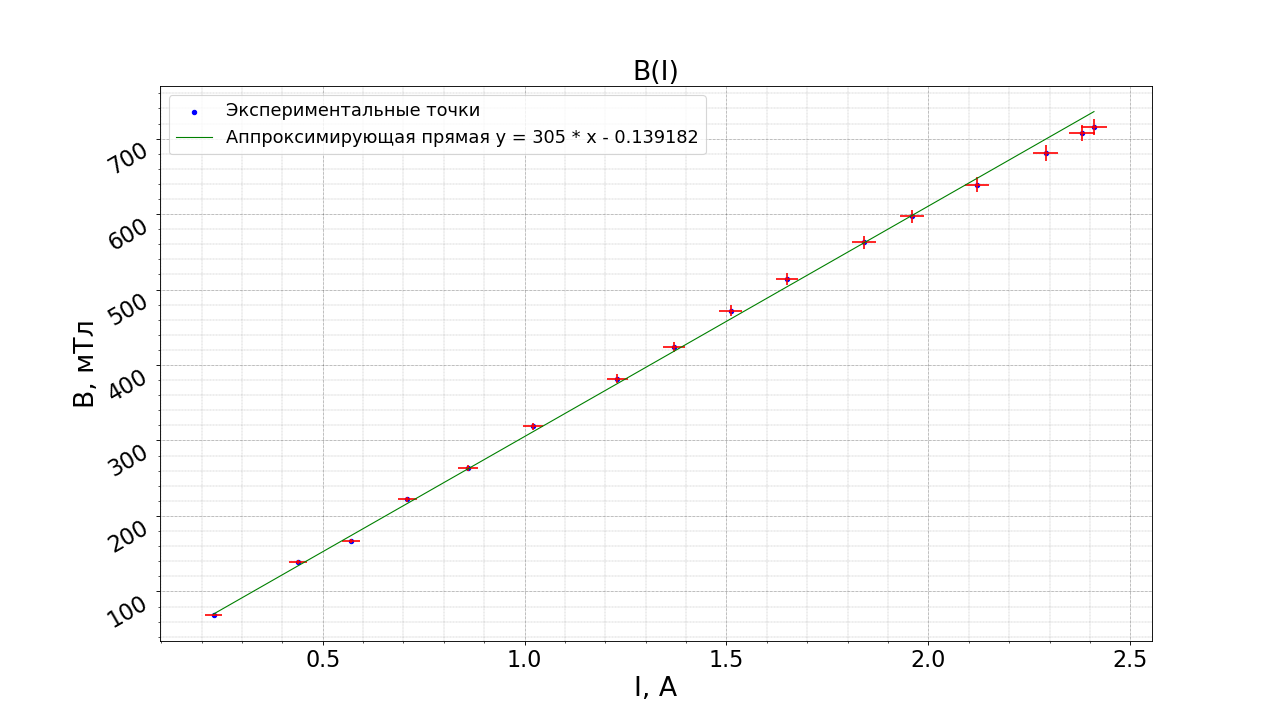
\includegraphics[width = 0.95\textwidth]{images/magnetic_field.png}
    \end{center}

    \noindent\hypertarget{graph_al}{\textbf{График 2. $|\Delta P| = f(B^2)$ для алюминия}}
    \begin{center}
        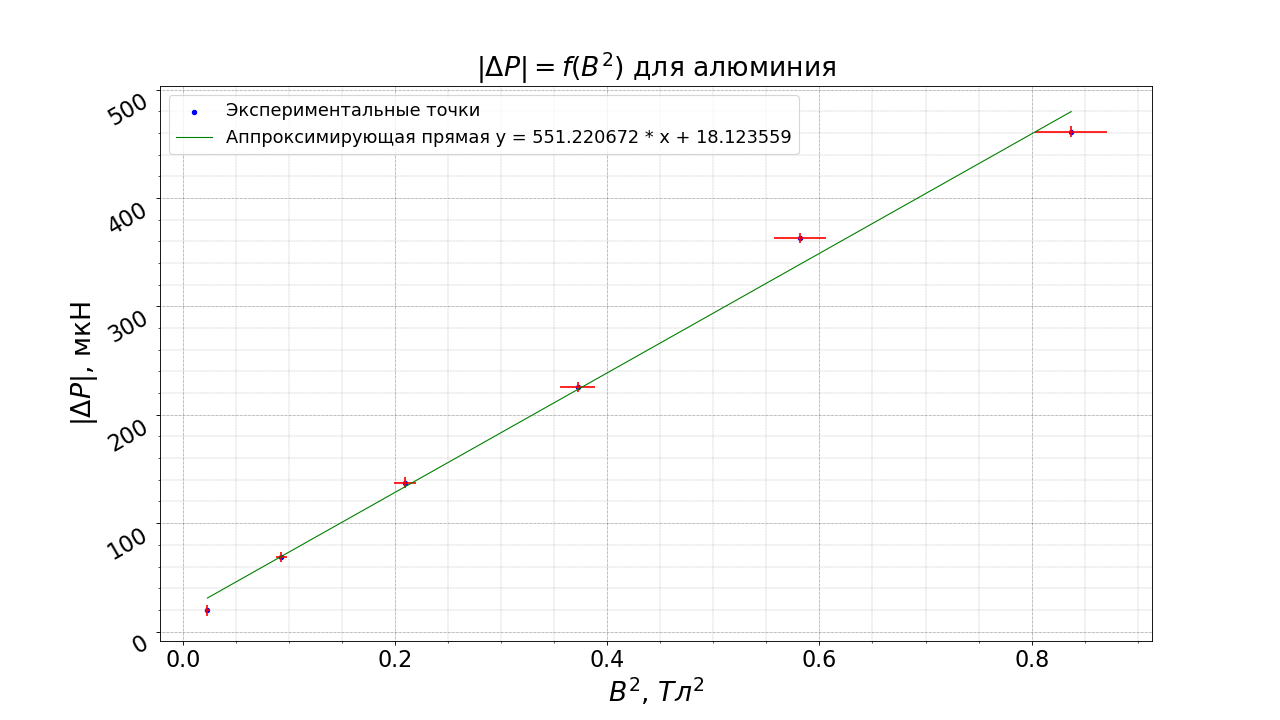
\includegraphics[width = 0.95\textwidth]{images/al.png}
    \end{center}

    \noindent\hypertarget{graph_cu}{\textbf{График 3. $|\Delta P| = f(B^2)$ для меди}}
    \begin{center}
        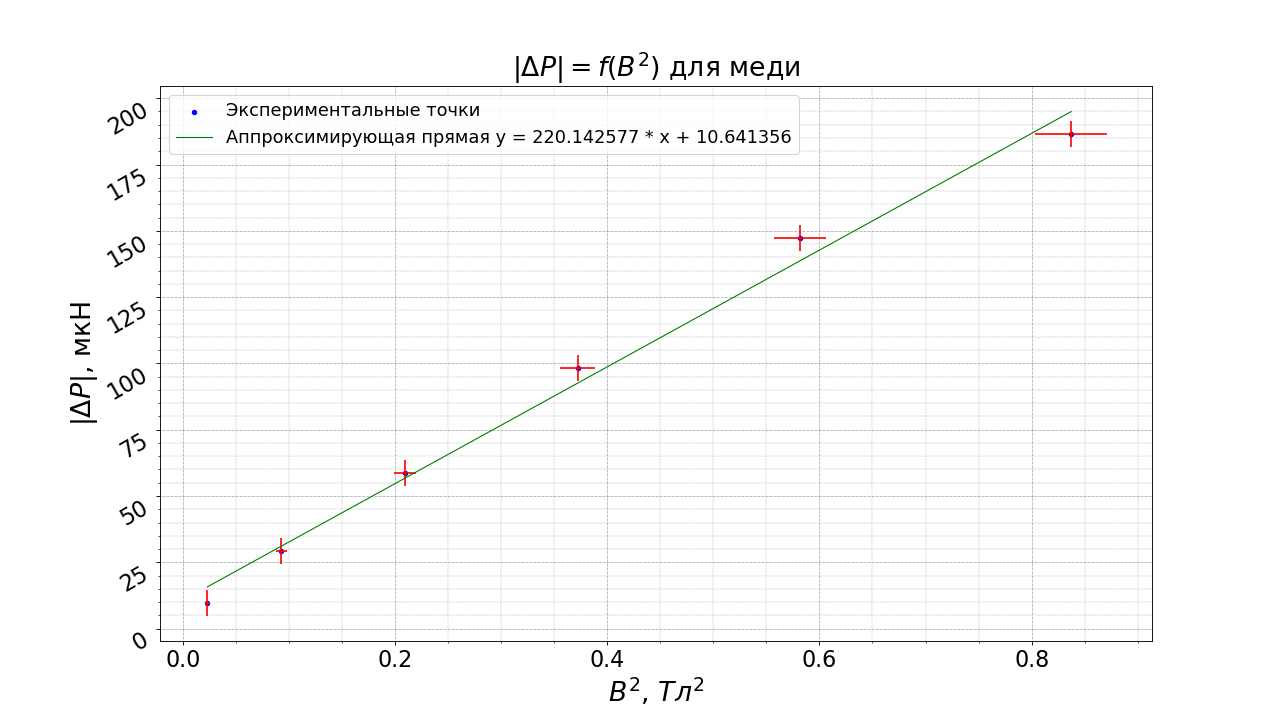
\includegraphics[width = \textwidth]{images/cu.png}
    \end{center}

    \noindent\hypertarget{graph_mix}{\textbf{График 4. $|\Delta P| = f(B^2)$ для алюминия и меди}}
    \begin{center}
        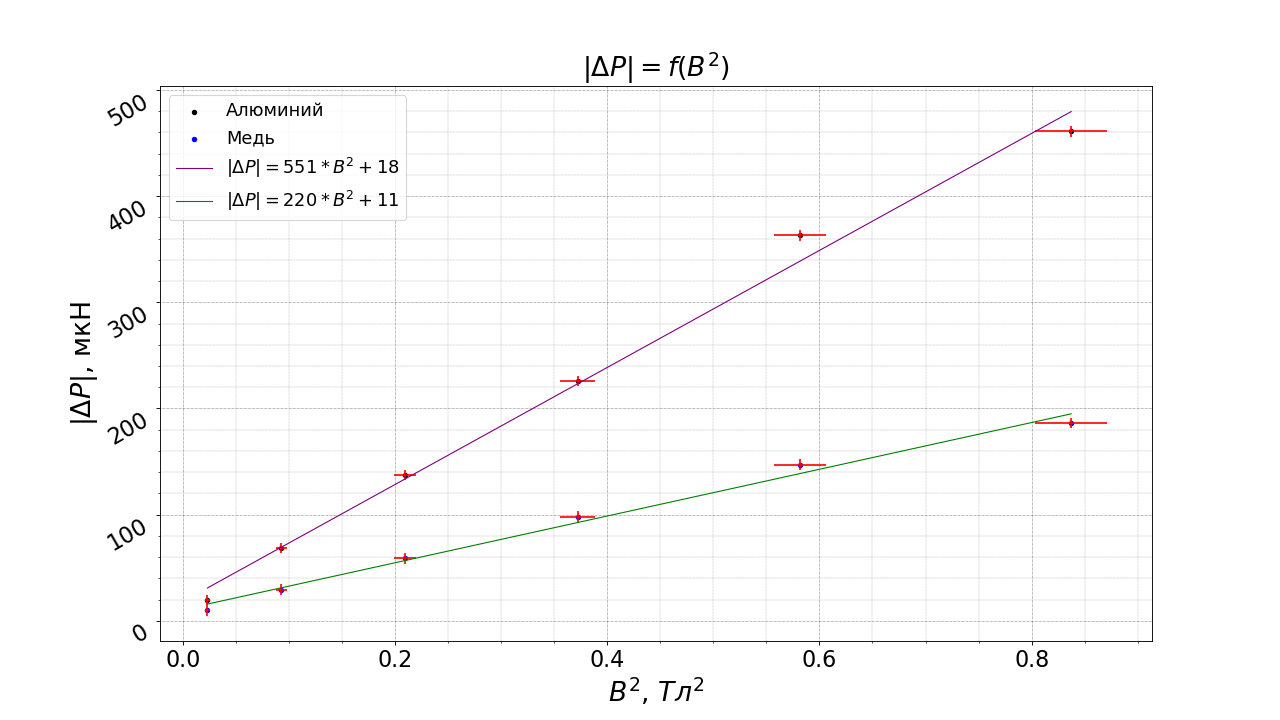
\includegraphics[width = \textwidth]{images/mix.png}
    \end{center}

\end{document}
